\documentclass[twoside,landscape,letterpaper,twocolumn,13pt]{book}

%landscape Para poner el documento en hojas horizontales

\usepackage{amsmath,amssymb,amsthm}
\usepackage{latexsym}
\usepackage[spanish]{babel}

\usepackage{graphicx}
%______________________________________
%               MARGENES
%______________________________________

\usepackage[scale=0.85]{geometry} 

%\usepackage[top = 1.65cm, bottom =1cm,left = 1.9cm,right = 1cm]{geometry} 

%______________________________________
%             ENCABEZADOS
%______________________________________
\usepackage{emptypage} % Quita encabezados y números de página de las paginas en blanco.

%______________________________________
%               COLUMNA
%______________________________________
\setlength{\columnsep}{0cm} %define la distancia entre las dos columnas

\setlength{\columnseprule}{0.5pt} %Configura la linea que separa las columnas

%______________________________________
%           ESPACIADO DE PARRAFO
%______________________________________

\parskip=4pt% Con carácter general la distancia entre párrafos está controlada por la variable \parskip que es una medida y por lo tanto se modifica simplemente asignándole un nuevo valor.

%______________________________________
%          ESPACIADO DE TEXTO
%______________________________________              
%Aumentar el espacio entre líneas (útil para correcciones)
%Para f = 1 => espaciado normal. 
%Para f = 1.3 => 1.5 espacios. 
%Para f = 1.6 => doble espacio.
\linespread{1}


%______________________________________
%         CONFIGURACION ENUMERATE
%______________________________________

%\renewcommand{\labelenumi}{\arabic{enumi}.}  % (1., 2., 3.,...)
%\renewcommand{\labelenumi}{\alph{enumi})} %(i., ii., iii.,...)
%\renewcommand{\theenumi}{\Roman{enumi}} % (I., II., III.,...)
%\renewcommand{\labelenumi}{\alph{enumi}.}    %(a., b., c.,...)
%\renewcommand{\labelenumi}{({\bf \alph{enumi}})}   %[(a), (b), (c),...]
%\renewcommand{\labelenumi}{\Alph{enumi}.}    %(A., B., C.,...)


%______________________________________
%             DOCUMENTO
%______________________________________

\begin{document}
\pagestyle{empty} %para que no aprezca el número de página en ninguna hoja.

\section*{Reglas básicas de derivación}

\begin{itemize}
    \item $(f\cdot g)^{'}(x)  = (f)^{'}(x) \cdot g(x) + g^{'}(x)  \cdot f(x)   $
    \item $\displaystyle{\left( \frac{f}{g} \right)}^{'}(x) =\displaystyle{\frac{ (f)^{'}(x) \cdot g(x) - g^{'}(x)  \cdot f(x)}{g^{2}(x)}}$
    \item $(\ln)^{'}(x) = \displaystyle{\frac{1}{x}}, \,\,\, x > 0 $
    \item $\sin^{'}(x) = \cos(x)$
    \item $\cos^{'}(x) = -\sen(x)$
    \item $\tan^{'}(x) = \sec^{2}(x)$
    \item $\sec^{'}(x) = \sec(x) \cdot \tan(x)$
    \item $\displaystyle{\frac{d}{dx}(\sin^{-1}(x))}= \displaystyle{\frac{1}{\sqrt{1-x^{2}}}, \,\,\,\, -1 <  x < 1 }$
    \item $\displaystyle{\frac{d}{dx}(\cos^{-1}(x))}= \displaystyle{- \frac{1}{\sqrt{1-x^{2}}}, \,\,\,\, -1 <  x < 1 }$

    \item $\displaystyle{\frac{d}{dx}(\tan^{-1}(x))} = \displaystyle{\frac{1}{1+x^{2}}, \,\,\,\, x \in \mathbb{R}}$
    
    \item $\displaystyle{\frac{d}{dx}(\sec^{-1}(x))} = \displaystyle{\frac{1}{|x| \sqrt{x^{2} - 1}}, \,\,\,\, |x| > 1}$
    
\end{itemize}

\section*{Regla de la cadena}
\begin{equation}
(f(g(x)))^{'} =\displaystyle{ f^{'}(g(x)) \cdot g^{'}(x)}
\end{equation}


\section*{Identidades trigonométricas}

\begin{itemize}
    \item $\displaystyle{\cos^{2}(\theta) = \frac{1+ \cos(2\theta)}{2}}$

    \item $\displaystyle{\sin^{2}(\theta) = \frac{1- \cos(2\theta)}{2}}$

    \item $1 + \tan^{2}(\theta) = \sec^{2}(\theta)$
    
\end{itemize}

\section*{Teorema del cambio de variable}

\begin{equation}
    \displaystyle{\int_{a}^{b} f(u(x))u^{'}(x) dx = \int_{u(a)}^{u(b)} f(u)du  }
\end{equation}


\section*{Reglas básicas de integración}

\begin{itemize}
    \item $\displaystyle{\int \frac{1}{\sqrt{a^{2} - x^{2}}} dx } = \sin^{-1}\left(\frac{x}{a}\right) + C, \, \, \, \, a >0$

    \item $\displaystyle{\int \frac{1}{a^{2} + x^{2}} dx } = \frac{1}{a} \tan^{-1}\left(\frac{x}{a}\right) + C, \,  \, \, \, a >0$

     \item $\displaystyle{\int \frac{1}{x\sqrt{x^{2} - a^{2}}}dx} = \frac{1}{a} \sec^{-1}\left(\frac{|x|}{a}\right) + C, \,  \, \, \, a >0$
     
\end{itemize}

\subsection*{Tabla de substituciones trigonométricas}

\begin{table}[t]
\begin{center}
\begin{tabular}{| r | c | c | c|}
\hline
Expresión & Susbtitución & Rango & Diferencia \\
\hline
$\sqrt{a^{2} - x^{2}}$ & $x = a \sin(\theta)$ & $-\frac{\pi}{2} \leq \theta \leq \frac{\pi}{2} $ & $dx = a \cos{\theta} d\theta$\\
 \hline
 $\sqrt{a^{2} + x^{2}}$ & $x = a \tan(\theta)$ & $-\frac{\pi}{2} < \theta < \frac{\pi}{2} $ & $dx = a \sec^{2}{\theta} d\theta$\\
 \hline
 $\sqrt{x^{2} -  a^{2}}$ & $x = a \sec(\theta)$ & $0 \leq \theta < \frac{\pi}{2}, \frac{\pi}{2} < \theta \leq \pi $ & $dx = a \sec{\theta}\tan{\theta} d\theta$\\
 \hline
\end{tabular}

\end{center}
\end{table}


\section*{Círculo unitario}
\centering{
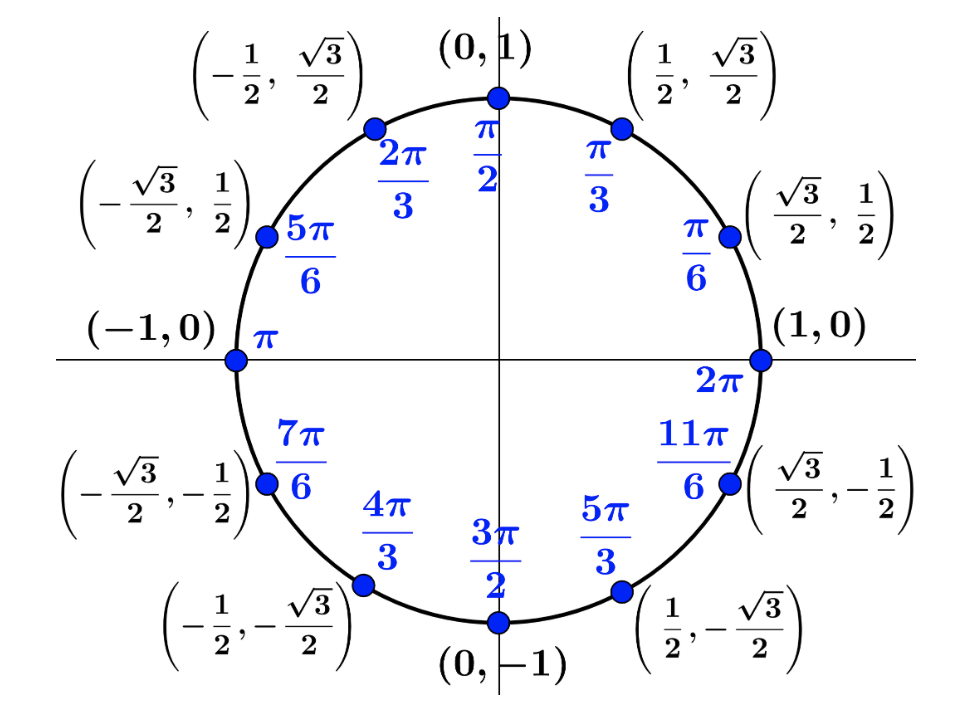
\includegraphics[width=0.35\textwidth]{Formulario/circulounitario.png}\par}

\end{document}